\subsection{Numerical Analysis}
\label{sec:numerical-reparameterization}

In this subsection we will use the data in \ref{subsec:synthetic-data-generation} perform reparameterization, classification and measure performance in terms of accuracy and computation time as the search size increases.

\FloatBarrier
\subsubsection{Reparameterization of Curves}
\label{subsec:reparameterization-curves}

In this subsection, we evaluate the reparameterization framework using synthetic curves generated previously (Section \ref{subsec:synthetic-data-generation}). The goal is to reparameterize the equidistantly parameterized curves \(c_i^\text{eq}\) into the curves \(c_i^j\) for \(i \in \{1, 2, 3\}\) and \(c_{i,i+1,i+2}^\text{eq}\) into the curves \(c_{i,i+1,i+2}^j\) for \(i \in \{1, 4, 7\}\), for all parameterizations \(j \in \{1, 2, 3\}\). This evaluation checks whether we can find the optimal reparameterization when the shapes are the same, demonstrating that we can effectively remove the effects of parameterization through reparameterization. It does not, however, determine whether we can differentiate between different shapes.

The objective is to find the optimal reparameterization \(\hat{\varphi}_j\) that approximates \(\varphi_j\). The relationship between the curves is given by:
\begin{equation}
    c_i^j = c_i^\text{eq} \circ \varphi_j
\end{equation}

Hence, each curve \(c_i^j\) is obtained by composing the equidistant curve \(c_i^\text{eq}\) with one of the parameterizations \(\varphi_1, \varphi_2\), or \(\varphi_3\). Thus, to find the optimal reparameterization \(\hat{\varphi}_j\), we minimize the distance \(d_{\mathcal{S}_*}\) between \(c_i^j\) and \(c_i^{\text{eq}}\):
\begin{equation}
    d_{\mathcal{S}_*}(c_i^j, c_i^{\text{eq}}) = \min_{\hat{\varphi}_j} d_{\mathcal{P}_*}(c_i^{\text{eq}} \circ \varphi_j, c_i^{\text{eq}} \circ \hat{\varphi}_j)
\end{equation}

This minimization process helps to determine \(\hat{\varphi}_j\) such that \(\hat{\varphi}_j \approx \varphi_j\), indicating that the reparameterization framework can effectively approximate the original parameterizations.

The results after reparameterization for the curves in \(\mathrm{SO}(3)\), \(\mathrm{SE}(3)\), \(\mathrm{SO}(3)^3\), and \(\mathrm{SE}(3)^3\) are presented in Figures \ref{fig:reparameterization-SO3}, \ref{fig:reparameterization-SE3}, \ref{fig:reparameterization-SO3-3}, and \ref{fig:reparameterization-SE3-3}, respectively.

\begin{figure}
    \begin{tikzpicture}
        \begin{axis}[
            width=0.85\textwidth,
            height=0.55\textwidth,
            xlabel={\( x \)},
            ylabel={\( \varphi(x) \)},
            grid=major,
            grid style={dashed,gray!30},
            legend style={at={(1.05,0.5)}, anchor=west},
            line width=1pt,
            xmin=0, xmax=1,
            ymin=0, ymax=1,
        ]
        \addplot [thin, red, solid] table [x=x, y=varphi_1, col sep=comma] {figures/syntetic_data/parameterization/varphi_1.csv};
        \addlegendentry{\( \varphi_1\)}

        \addplot [thin, blue, solid] table [x=x, y=varphi_2, col sep=comma] {figures/syntetic_data/parameterization/varphi_2.csv};
        \addlegendentry{\( \varphi_2\)}

        \addplot [thin, green, solid] table [x=x, y=varphi_3, col sep=comma] {figures/syntetic_data/parameterization/varphi_3.csv};
        \addlegendentry{\( \varphi_3\)}


        \addplot [red, dashed] table [x=x, y=g0, col sep=comma] {figures/syntetic_data/reparameterization_SO3/df_varphi_1.csv};
        \addlegendentry{\( \hat \varphi_{1}^{1}\)}

        \addplot [red, dotted] table [x=x, y=g1, col sep=comma] {figures/syntetic_data/reparameterization_SO3/df_varphi_1.csv};
        \addlegendentry{\( \hat \varphi_{1}^{2}\)}

        \addplot [red, dashdotted] table [x=x, y=g2, col sep=comma] {figures/syntetic_data/reparameterization_SO3/df_varphi_1.csv};
        \addlegendentry{\( \hat \varphi_{1}^{3}\)}

        \addplot [blue, dashed] table [x=x, y=g0, col sep=comma] {figures/syntetic_data/reparameterization_SO3/df_varphi_2.csv};
        \addlegendentry{\( \hat \varphi_{2}^{1}\)}

        \addplot [blue, dotted] table [x=x, y=g1, col sep=comma] {figures/syntetic_data/reparameterization_SO3/df_varphi_2.csv};
        \addlegendentry{\( \hat \varphi_{2}^{2}\)}

        \addplot [blue, dashdotted] table [x=x, y=g2, col sep=comma] {figures/syntetic_data/reparameterization_SO3/df_varphi_2.csv};
        \addlegendentry{\( \hat \varphi_{2}^{3}\)}

        \addplot [green, dashed] table [x=x, y=g0, col sep=comma] {figures/syntetic_data/reparameterization_SO3/df_varphi_3.csv};
        \addlegendentry{\( \hat \varphi_{3}^{1}\)}

        \addplot [green, dotted] table [x=x, y=g1, col sep=comma] {figures/syntetic_data/reparameterization_SO3/df_varphi_3.csv};
        \addlegendentry{\( \hat \varphi_{3}^{2}\)}

        \addplot [green, dashdotted] table [x=x, y=g2, col sep=comma] {figures/syntetic_data/reparameterization_SO3/df_varphi_3.csv};
        \addlegendentry{\( \hat \varphi_{3}^{3}\)}

        \end{axis}
    \end{tikzpicture}    
    \caption[Reparameterization of curves in \(\mathrm{SO}(3)\)]{Comparison of reparameterized curves \(\hat{\varphi}_j^i\) with the analytical parameterizations \(\varphi_j\) for curves in \(\mathrm{SO}(3)\). The curves \(c_i^{\text{eq}}\) have been fitted to \(c_i^j\) for \(j = 1, 2, 3\), and for all shapes \(i = 1, 2, 3\). Optimal reparameterizations are indicated by \(\hat{\varphi}_i^j\) being close to \(\varphi_j\).}
    \label{fig:reparameterization-SO3}
\end{figure}

\begin{figure}
    \begin{tikzpicture}
        \begin{axis}[
            width=0.85\textwidth,
            height=0.55\textwidth,
            xlabel={\( x \)},
            ylabel={\( \varphi(x) \)},
            grid=major,
            grid style={dashed,gray!30},
            legend style={at={(1.05,0.5)}, anchor=west},
            line width=1pt,
            xmin=0, xmax=1,
            ymin=0, ymax=1,
        ]
        \addplot [thin, red, solid] table [x=x, y=varphi_1, col sep=comma] {figures/syntetic_data/parameterization/varphi_1.csv};
        \addlegendentry{\( \varphi_1\)}

        \addplot [thin, blue, solid] table [x=x, y=varphi_2, col sep=comma] {figures/syntetic_data/parameterization/varphi_2.csv};
        \addlegendentry{\( \varphi_2\)}

        \addplot [thin, green, solid] table [x=x, y=varphi_3, col sep=comma] {figures/syntetic_data/parameterization/varphi_3.csv};
        \addlegendentry{\( \varphi_3\)}

        \addplot [red, dashed] table [x=x, y=g0, col sep=comma] {figures/syntetic_data/reparameterization_SE3/df_varphi_1.csv};
        \addlegendentry{\( \hat \varphi_{1}^1\)}

        \addplot [red, dotted] table [x=x, y=g1, col sep=comma] {figures/syntetic_data/reparameterization_SE3/df_varphi_1.csv};
        \addlegendentry{\( \hat \varphi_{1}^2\)}

        \addplot [red, dashdotted] table [x=x, y=g2, col sep=comma] {figures/syntetic_data/reparameterization_SE3/df_varphi_1.csv};
        \addlegendentry{\( \hat \varphi_{1}^3\)}

        \addplot [blue, dashed] table [x=x, y=g0, col sep=comma] {figures/syntetic_data/reparameterization_SE3/df_varphi_2.csv};
        \addlegendentry{\( \hat \varphi_{2}^1\)}

        \addplot [blue, dotted] table [x=x, y=g1, col sep=comma] {figures/syntetic_data/reparameterization_SE3/df_varphi_2.csv};
        \addlegendentry{\( \hat \varphi_{2}^2\)}

        \addplot [blue, dashdotted] table [x=x, y=g2, col sep=comma] {figures/syntetic_data/reparameterization_SE3/df_varphi_2.csv};
        \addlegendentry{\( \hat \varphi_{2}^3\)}

        \addplot [green, dashed] table [x=x, y=g0, col sep=comma] {figures/syntetic_data/reparameterization_SE3/df_varphi_3.csv};
        \addlegendentry{\( \hat \varphi_{3}^1\)}

        \addplot [green, dotted] table [x=x, y=g1, col sep=comma] {figures/syntetic_data/reparameterization_SE3/df_varphi_3.csv};
        \addlegendentry{\( \hat \varphi_{3}^2\)}

        \addplot [green, dashdotted] table [x=x, y=g2, col sep=comma] {figures/syntetic_data/reparameterization_SE3/df_varphi_3.csv};
        \addlegendentry{\( \hat \varphi_{3}^3\)}

        \end{axis}
    \end{tikzpicture}    
    \caption[Reparameterization of curves in \(\mathrm{SE}(3)\)]{Comparison of reparameterized curves \(\hat{\varphi}_j^i\) with the analytical parameterizations \(\varphi_j\) for curves in \(\mathrm{SE}(3)\). The curves \(c_i^{\text{eq}}\) have been fitted to \(c_i^j\) for \(j = 1, 2, 3\), and for all shapes \(i = 1, 2, 3\). Optimal reparameterizations are indicated by \(\hat{\varphi}_j^i\) being close to \(\varphi_j\).}
    \label{fig:reparameterization-SE3}
\end{figure}

\begin{figure}
    \begin{tikzpicture}
        \begin{axis}[
            width=0.8\textwidth,
            height=0.55\textwidth,
            xlabel={\( x \)},
            ylabel={\( \varphi(x) \)},
            grid=major,
            grid style={dashed,gray!30},
            legend style={at={(1.05,0.5)}, anchor=west},
            line width=1pt,
            xmin=0, xmax=1,
            ymin=0, ymax=1,
        ]
        \addplot [thin, red, solid] table [x=x, y=varphi_1, col sep=comma] {figures/syntetic_data/parameterization/varphi_1.csv};
        \addlegendentry{\( \varphi_1\)}

        \addplot [thin, blue, solid] table [x=x, y=varphi_2, col sep=comma] {figures/syntetic_data/parameterization/varphi_2.csv};
        \addlegendentry{\( \varphi_2\)}

        \addplot [thin, green, solid] table [x=x, y=varphi_3, col sep=comma] {figures/syntetic_data/parameterization/varphi_3.csv};
        \addlegendentry{\( \varphi_3\)}


        \addplot [red, dashed] table [x=x, y=g0, col sep=comma] {figures/syntetic_data/reparameterization_SO3_3/df_varphi_1.csv};
        \addlegendentry{\( \hat \varphi_{1}^{(1,2,3)}\)}

        \addplot [red, dotted] table [x=x, y=g1, col sep=comma] {figures/syntetic_data/reparameterization_SO3_3/df_varphi_1.csv};
        \addlegendentry{\( \hat \varphi_{1}^{(4,5,6)}\)}

        \addplot [red, dashdotted] table [x=x, y=g2, col sep=comma] {figures/syntetic_data/reparameterization_SO3_3/df_varphi_1.csv};
        \addlegendentry{\( \hat \varphi_{1}^{(7,8,9)}\)}

        \addplot [blue, dashed] table [x=x, y=g0, col sep=comma] {figures/syntetic_data/reparameterization_SO3_3/df_varphi_2.csv};
        \addlegendentry{\( \hat \varphi_{2}^{(1,2,3)}\)}

        \addplot [blue, dotted] table [x=x, y=g1, col sep=comma] {figures/syntetic_data/reparameterization_SO3_3/df_varphi_2.csv};
        \addlegendentry{\( \hat \varphi_{2}^{(4,5,6)}\)}

        \addplot [blue, dashdotted] table [x=x, y=g2, col sep=comma] {figures/syntetic_data/reparameterization_SO3_3/df_varphi_2.csv};
        \addlegendentry{\( \hat \varphi_{2}^{(7,8,9)}\)}

        \addplot [green, dashed] table [x=x, y=g0, col sep=comma] {figures/syntetic_data/reparameterization_SO3_3/df_varphi_3.csv};
        \addlegendentry{\( \hat \varphi_{3}^{(1,2,3)}\)}

        \addplot [green, dotted] table [x=x, y=g1, col sep=comma] {figures/syntetic_data/reparameterization_SO3_3/df_varphi_3.csv};
        \addlegendentry{\( \hat \varphi_{3}^{(4,5,6)}\)}

        \addplot [green, dashdotted] table [x=x, y=g2, col sep=comma] {figures/syntetic_data/reparameterization_SO3_3/df_varphi_3.csv};
        \addlegendentry{\( \hat \varphi_{3}^{(7,8,9)}\)}
        \end{axis}
    \end{tikzpicture}    
    \caption[Reparameterization of curves in \(\mathrm{SO}(3)^3\)]{Comparison of reparameterized curves \(\hat{\varphi}_j^{i,i+1,i+2}\) with the analytical parameterizations \(\varphi_j\) for curves in \(\mathrm{SE}(3)\). The curves \(c_{i,i+1,i+2}^{\text{eq}}\) have been fitted to \(c_{i,i+1,i+2}^j\) for \(i \in \{1, 2, 3\}\), and for all shapes \(i \in \{1, 4, 7\}\). Optimal reparameterizations are indicated by \(\hat{\varphi}_j^{i,i+1,i+2}\) being close to \(\varphi_j\).}
    \label{fig:reparameterization-SO3-3}
\end{figure}

\begin{figure}
    \begin{tikzpicture}
        \begin{axis}[
            width=0.8\textwidth,
            height=0.55\textwidth,
            xlabel={\( x \)},
            ylabel={\( \varphi(x) \)},
            grid=major,
            grid style={dashed,gray!30},
            legend style={at={(1.05,0.5)}, anchor=west},
            line width=1pt,
            xmin=0, xmax=1,
            ymin=0, ymax=1,
        ]
        \addplot [thin, red, solid] table [x=x, y=varphi_1, col sep=comma] {figures/syntetic_data/parameterization/varphi_1.csv};
        \addlegendentry{\( \varphi_1\)}

        \addplot [thin, blue, solid] table [x=x, y=varphi_2, col sep=comma] {figures/syntetic_data/parameterization/varphi_2.csv};
        \addlegendentry{\( \varphi_2\)}

        \addplot [thin, green, solid] table [x=x, y=varphi_3, col sep=comma] {figures/syntetic_data/parameterization/varphi_3.csv};
        \addlegendentry{\( \varphi_3\)}



        \addplot [red, dashed] table [x=x, y=g0, col sep=comma] {figures/syntetic_data/reparameterization_SE3_3/df_varphi_1.csv};
        \addlegendentry{\( \hat \varphi_{1}^{(1,2,3)}\)}

        \addplot [red, dotted] table [x=x, y=g1, col sep=comma] {figures/syntetic_data/reparameterization_SE3_3/df_varphi_1.csv};
        \addlegendentry{\( \hat \varphi_{1}^{(4,5,6)}\)}

        \addplot [red, dashdotted] table [x=x, y=g2, col sep=comma] {figures/syntetic_data/reparameterization_SE3_3/df_varphi_1.csv};
        \addlegendentry{\( \hat \varphi_{1}^{(7,8,9)}\)}

        \addplot [blue, dashed] table [x=x, y=g0, col sep=comma] {figures/syntetic_data/reparameterization_SE3_3/df_varphi_2.csv};
        \addlegendentry{\( \hat \varphi_{2}^{(1,2,3)}\)}

        \addplot [blue, dotted] table [x=x, y=g1, col sep=comma] {figures/syntetic_data/reparameterization_SE3_3/df_varphi_2.csv};
        \addlegendentry{\( \hat \varphi_{2}^{(4,5,6)}\)}

        \addplot [blue, dashdotted] table [x=x, y=g2, col sep=comma] {figures/syntetic_data/reparameterization_SE3_3/df_varphi_2.csv};
        \addlegendentry{\( \hat \varphi_{2}^{(7,8,9)}\)}

        \addplot [green, dashed] table [x=x, y=g0, col sep=comma] {figures/syntetic_data/reparameterization_SE3_3/df_varphi_3.csv};
        \addlegendentry{\( \hat \varphi_{3}^{(1,2,3)}\)}

        \addplot [green, dotted] table [x=x, y=g1, col sep=comma] {figures/syntetic_data/reparameterization_SE3_3/df_varphi_3.csv};
        \addlegendentry{\( \hat \varphi_{3}^{(4,5,6)}\)}

        \addplot [green, dashdotted] table [x=x, y=g2, col sep=comma] {figures/syntetic_data/reparameterization_SE3_3/df_varphi_3.csv};
        \addlegendentry{\( \hat \varphi_{3}^{(7,8,9)}\)}

        \end{axis}
    \end{tikzpicture}    
    \caption[Reparameterization of curves in \(\mathrm{SE}(3)^3\)]{Comparison of reparameterized curves \(\hat{\varphi}_j^{i,i+1,i+2}\) with the analytical parameterizations \(\varphi_j\) for curves in \(\mathrm{SE}(3)\). The curves \(c_{i,i+1,i+2}^{\text{eq}}\) have been fitted to \(c_{i,i+1,i+2}^j\) for \(j \in \{1, 2, 3\}\), and for all shapes \(i \in \{1, 4, 7\}\). Optimal reparameterizations are indicated by \(\hat{\varphi}_j^{i,i+1,i+2}\) being close to \(\varphi_j\).}
    \label{fig:reparameterization-SE3-3}
\end{figure}

The reparameterization results show that the optimal reparameterizations \(\hat{\varphi}_j^i\) for \(i \in \{1, 2, 3\}\) and \(\hat{\varphi}_j^{i,i+1,i+2}\) for \(i \in \{1, 4, 7\}\) closely approximate the original parameterizations \(\varphi_j\) for all \(j \in \{1, 2, 3\}\). This indicates that our framework can effectively remove the effects of parameterization. The results are consistent across all groups, attesting to its robustness. However, this evaluation only verifies the ability to find the parameterization for curves with the same shape. 

Overall, the results affirm the reparameterization framework's effectiveness in approximating original parameterizations and suggest its potential for broader applications in shape analysis and related fields.

\FloatBarrier
\subsubsection{Classification of Curves}
\label{subsec:classification-curves}

The primary objective here is to classify curves based on their geometric shapes using our reparameterization framework. This classification utilizes the curves generated in Section \ref{subsec:synthetic-data-generation}. Specifically, we use the curves \(c_i^j\) and \(c_i^{\text{eq}}\) for \(\mathrm{SO}(3)\) and \(\mathrm{SE}(3)\), as well as \(c_{i,i+1,i+2}^j\) and \(c_{i,i+1,i+2}^{\text{eq}}\) for \(\mathrm{SO}(3)^3\) and \(\mathrm{SE}(3)^3\). Our framework aims to find the shape space metric \(d_{\mathcal{S}_*}\), as defined in Equation \eqref{eq:shape-space-metric-id}, between these curves to create a distance matrix. Instead of directly classifying the curves, we visualize the distances to observe clustering of similar shapes and separation of different shapes.

The color map of this matrix highlights the effectiveness of shape-based classification. We expect a block diagonal pattern in the matrix, with three 4x4 blocks along the diagonal indicating lower distances and thus, shape similarities. Conversely, the off-diagonal blocks should display higher, relatively uniform distances, suggesting distinct shapes. This pattern would confirm successful classification based on shape reparameterization, showing that geometrically similar curves cluster together, while different shapes are well-separated. 

\begin{figure}
    \centering
    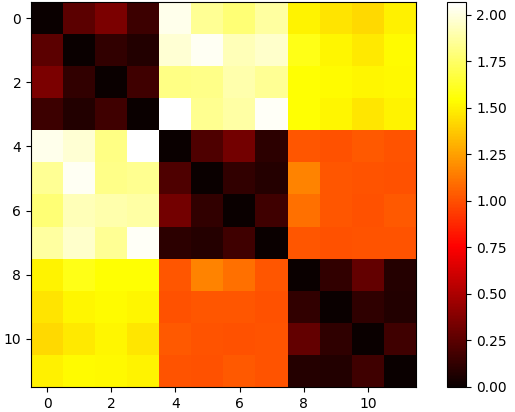
\includegraphics[width=0.7\linewidth]{figures/syntetic_data/distance_matrix/SO3.png}
    \caption[Classification using reparameterization of curves in \(\mathrm{SO}(3)\)]{Heat map of the distance matrix for twelve synthetic \(\mathrm{SO}(3)\) curves, denoted \(c_i^j\), where \(i \in \{1, 2, 3\}\) indicates the shape and \(j \in \{1, 2, 3, \text{eq}\}\) represents the parameterization. The color intensity reflects the shape space distance, with lower distances indicating similarity in shape and higher distances signifying distinct shapes.}
    \label{fig:classification-SO3}
\end{figure}

\begin{figure}
    \centering
    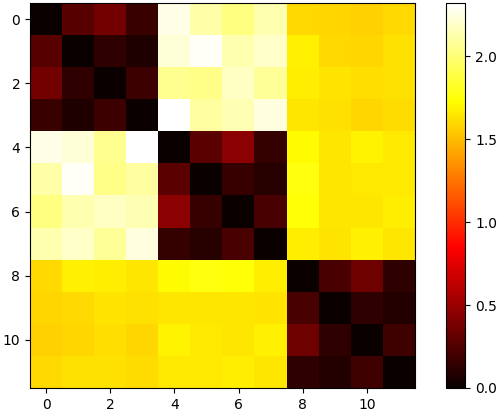
\includegraphics[width=0.7\linewidth]{figures/syntetic_data/distance_matrix/SE3.png}
    \caption[Classification using reparameterization of curves in \(\mathrm{SE}(3)\)]{Heat map of the distance matrix for twelve synthetic \(\mathrm{SE}(3)\) curves, denoted \(c_i^j\), where \(i \in \{1, 2, 3\}\) indicates the shape and \(j \in \{1, 2, 3, \text{eq}\}\) represents the parameterization. The color intensity reflects the shape space distance, with lower distances indicating similarity in shape and higher distances signifying distinct shapes.}
    \label{fig:classification-SE3}
\end{figure}

\begin{figure}
    \centering
    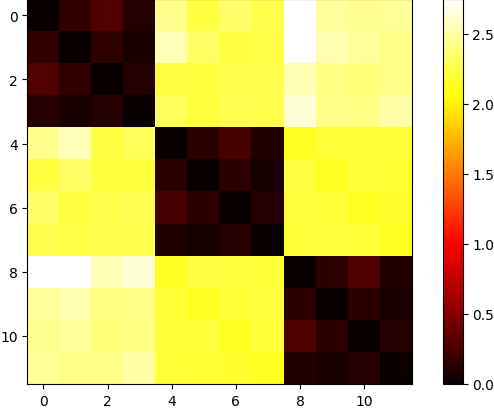
\includegraphics[width=0.7\linewidth]{figures/syntetic_data/distance_matrix/SO3_3.png}
    \caption[Classification using reparameterization of curves in \(\mathrm{SO}(3)^3\)]{Heat map of the distance matrix for twelve synthetic \(\mathrm{SO}(3)^3\) curves, denoted \(c_{(i,i+1,i+2)}^j\), where \(i \in \{1, 4, 7\}\) indicates the shape and \(j \in \{1, 2, 3, \text{eq}\}\) represents the parameterization. The color intensity reflects the shape space distance, with lower distances indicating similarity in shape and higher distances signifying distinct shapes.}
    \label{fig:classification-SO3-3}
\end{figure}

\begin{figure}
    \centering
    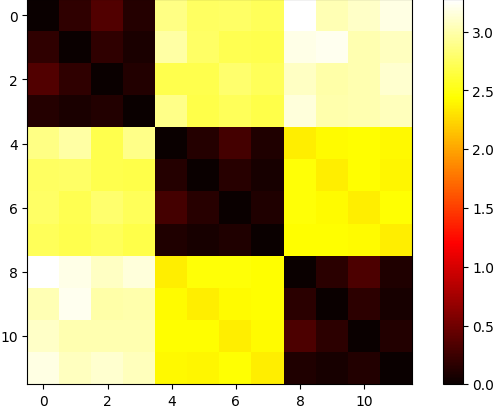
\includegraphics[width=0.7\linewidth]{figures/syntetic_data/distance_matrix/SE3_3.png}
    \caption[Classification using reparameterization of curves in \(\mathrm{SE}(3)^3\)]{Heat map of the distance matrix for twelve synthetic \(\mathrm{SE}(3)^3\) curves, denoted \(c_{(i,i+1,i+2)}^j\), where \(i \in \{1, 4, 7\}\) indicates the shape and \(j \in \{1, 2, 3, \text{eq}\}\) represents the parameterization. The color intensity reflects the shape space distance, with lower distances indicating similarity in shape and higher distances signifying distinct shapes.}
    \label{fig:classification-SE3-3}
\end{figure}

The classification outcomes for each dataset type \(\mathrm{SO}(3)\), \(\mathrm{SE}(3)\), \(\mathrm{SO}(3)^3\), and \(\mathrm{SE}(3)^3\) are depicted in Figures \ref{fig:classification-SO3}, \ref{fig:classification-SE3}, \ref{fig:classification-SO3-3}, and \ref{fig:classification-SE3-3}, respectively. These results highlight the efficacy of our methodology in distinguishing between curve shapes through reparameterization, demonstrating the robustness and utility of the proposed approach.

Notably, the classification is more precise for curves in \(\mathrm{SO}(3)^3\) and \(\mathrm{SE}(3)^3\). In these cases, the distances between curves of the same shape are significantly closer, while distances between curves of different shapes are more pronounced compared to those in \(\mathrm{SO}(3)\) and \(\mathrm{SE}(3)\). This suggests that our reparameterization framework is particularly effective in higher-dimensional settings, where it can better capture and distinguish subtle geometric differences.

\FloatBarrier
\subsubsection{Reduced Search Area}
\label{subsubsec:reduced-search-area}

In practical applications, exhaustive domain searches can be computationally demanding, as outlined in Subsection \ref{subsec:neighborhood-search-strategy}. This becomes impractical for large datasets or higher-dimensional spaces. To address this, we evaluate the impact of varying search depths on performance while maintaining a constant sample count. Our goal is to balance computational efficiency and accuracy by optimizing the search depth.

Figures \ref{fig:depth-error-single} and \ref{fig:depth-error-cartesian}, shows that the error decreases with increasing search depth across curves in \(\mathrm{SO}(3)\), \(\mathrm{SE}(3)\), \(\mathrm{SO}(3)^3\), and \(\mathrm{SE}(3)^3\). Initially, the error reduction is rapid, but it levels off as depth increases, with minimal differences observed between depths 4 and 10. This suggests diminishing returns in error reduction beyond a certain depth, which appears to be around search depth 4 for this dataset.

Figure \ref{fig:depth-error-time} illustrates the computation time required for these calculations. As expected, computation time increases significantly with greater search depth, though the growth is not strictly quadratic due to various operational efficiencies and the moderate scale of \(n\). These results highlight the need for an optimal search depth to balance accuracy and computational cost.

Based on these observations, we find that a search depth of 4 significantly reduces computation time while maintaining an acceptable error rate. This depth provides a practical balance between computational efficiency and accuracy, making it suitable for our reparameterization framework in both lower and higher-dimensional spaces. However, these findings are specific to the current dataset and may vary with different datasets.

\begin{figure}
    \centering
    \begin{subfigure}[c]{\textwidth}
        \begin{tikzpicture}
            \begin{axis}[
                width=0.8\textwidth,
                height=0.5\textwidth,
                ytick={0,1,2},
                xlabel={Search Depth},
                ylabel={\(d_{\mathcal{S}_*}\left(c^j, c^{\text{eq}}\right)\)},
                legend style={at={(1.05,0.5)}, anchor=west},
                grid=major,
            ]
            \addplot [thick, red, solid] table [x=depth, y=L2_distance, col sep=comma] {figures/syntetic_data/reparameterization_SO3/depth_error/g0_varphi0.csv};
            \addlegendentry{$c_1^1$}
    
            \addplot [thick, red, dashed] table [x=depth, y=L2_distance, col sep=comma] {figures/syntetic_data/reparameterization_SO3/depth_error/g0_varphi1.csv};
            \addlegendentry{$c_1^2$}
    
            \addplot [thick, red, dotted] table [x=depth, y=L2_distance, col sep=comma] {figures/syntetic_data/reparameterization_SO3/depth_error/g0_varphi2.csv};
            \addlegendentry{$c_1^3$}
    
            \addplot [thick, blue, solid] table [x=depth, y=L2_distance, col sep=comma] {figures/syntetic_data/reparameterization_SO3/depth_error/g1_varphi0.csv};
            \addlegendentry{$c_2^1$}
    
            \addplot [thick, blue, dashed] table [x=depth, y=L2_distance, col sep=comma] {figures/syntetic_data/reparameterization_SO3/depth_error/g1_varphi1.csv};
            \addlegendentry{$c_2^2$}
    
            \addplot [thick, blue, dotted] table [x=depth, y=L2_distance, col sep=comma] {figures/syntetic_data/reparameterization_SO3/depth_error/g1_varphi2.csv};
            \addlegendentry{$c_2^3$}
    
            \addplot [thick, green, solid] table [x=depth, y=L2_distance, col sep=comma] {figures/syntetic_data/reparameterization_SO3/depth_error/g2_varphi0.csv};
            \addlegendentry{$c_3^1$}
    
            \addplot [thick, green, dashed] table [x=depth, y=L2_distance, col sep=comma] {figures/syntetic_data/reparameterization_SO3/depth_error/g2_varphi1.csv};
            \addlegendentry{$c_3^2$}
    
            \addplot [thick, green, dotted] table [x=depth, y=L2_distance, col sep=comma] {figures/syntetic_data/reparameterization_SO3/depth_error/g2_varphi2.csv};
            \addlegendentry{$c_3^3$}
    
            \end{axis}
        \end{tikzpicture}
        \caption{}
    \end{subfigure}

    \centering
    \begin{subfigure}[c]{\textwidth}
        \begin{tikzpicture}
            \begin{axis}[
                width=0.8\textwidth,
                height=0.5\textwidth,
                xlabel={Search Depth},
                ylabel={\(d_{\mathcal{S}_*}\left(c^j, c^{\text{eq}}\right)\)},
                legend style={at={(1.05,0.5)}, anchor=west},
                grid=major,
            ]
            \addplot [thick, red, solid] table [x=depth, y=L2_distance, col sep=comma] {figures/syntetic_data/reparameterization_SE3/depth_error/g0_varphi0.csv};
            \addlegendentry{$c_1^1$}
    
            \addplot [thick, red, dashed] table [x=depth, y=L2_distance, col sep=comma] {figures/syntetic_data/reparameterization_SE3/depth_error/g0_varphi1.csv};
            \addlegendentry{$c_1^2$}
    
            \addplot [thick, red, dotted] table [x=depth, y=L2_distance, col sep=comma] {figures/syntetic_data/reparameterization_SE3/depth_error/g0_varphi2.csv};
            \addlegendentry{$c_1^3$}
    
            \addplot [thick, blue, solid] table [x=depth, y=L2_distance, col sep=comma] {figures/syntetic_data/reparameterization_SE3/depth_error/g1_varphi0.csv};
            \addlegendentry{$c_2^1$}
    
            \addplot [thick, blue, dashed] table [x=depth, y=L2_distance, col sep=comma] {figures/syntetic_data/reparameterization_SE3/depth_error/g1_varphi1.csv};
            \addlegendentry{$c_2^2$}
    
            \addplot [thick, blue, dotted] table [x=depth, y=L2_distance, col sep=comma] {figures/syntetic_data/reparameterization_SE3/depth_error/g1_varphi2.csv};
            \addlegendentry{$c_2^3$}
    
            \addplot [thick, green, solid] table [x=depth, y=L2_distance, col sep=comma] {figures/syntetic_data/reparameterization_SE3/depth_error/g2_varphi0.csv};
            \addlegendentry{$c_3^1$}
    
            \addplot [thick, green, dashed] table [x=depth, y=L2_distance, col sep=comma] {figures/syntetic_data/reparameterization_SE3/depth_error/g2_varphi1.csv};
            \addlegendentry{$c_3^2$}
    
            \addplot [thick, green, dotted] table [x=depth, y=L2_distance, col sep=comma] {figures/syntetic_data/reparameterization_SE3/depth_error/g2_varphi2.csv};
            \addlegendentry{$c_3^3$}
    
            \end{axis}
        \end{tikzpicture}
        \caption{}
    \end{subfigure}
    \caption[Convergence of Shape Distance with Increasing Search Depth in \(\mathrm{SO}(3)\) and \(\mathrm{SE}(3)\)]{Plot showing the convergence of shape distance \(d_{\mathcal{S}_*}\) (defined in Equation \eqref{eq:shape-space-metric-id}) between curve \(c_{i}^{\mathrm{eq}}\) and its reparameterization \(c_{i}^{j}\) for \(j \in \{1, 2, 3\}\) and \(i \in \{1, 2, 3\}\) within group \(G\) as search depth increases: (a) \(G = \mathrm{SO}(3)\), (b) \(G = \mathrm{SE}(3)\).}
    \label{fig:depth-error-single}
\end{figure}

\begin{figure}
    \centering
    \begin{subfigure}[c]{\textwidth}
        \begin{tikzpicture}
            \begin{axis}[
                width=0.8\textwidth,
                height=0.5\textwidth,
                xlabel={Search Depth},
                ylabel={\(d_{\mathcal{S}_*}\left(c^j, c^{\text{eq}}\right)\)},
                legend style={at={(1.05,0.5)}, anchor=west},
                grid=major,
            ]
            \addplot [thick, red, solid] table [x=depth, y=L2_distance, col sep=comma] {figures/syntetic_data/reparameterization_SO3_3/depth_error/g0_varphi0.csv};
            \addlegendentry{$c_{(1,2,3)}^1$}
    
            \addplot [thick, red, dashed] table [x=depth, y=L2_distance, col sep=comma] {figures/syntetic_data/reparameterization_SO3_3/depth_error/g0_varphi1.csv};
            \addlegendentry{$c_{(1,2,3)}^2$}
    
            \addplot [thick, red, dotted] table [x=depth, y=L2_distance, col sep=comma] {figures/syntetic_data/reparameterization_SO3_3/depth_error/g0_varphi2.csv};
            \addlegendentry{$c_{(1,2,3)}^3$}

            \addplot [thick, blue, solid] table [x=depth, y=L2_distance, col sep=comma] {figures/syntetic_data/reparameterization_SO3_3/depth_error/g1_varphi0.csv};
            \addlegendentry{$c_{(4,5,6)}^1$}
    
            \addplot [thick, blue, dashed] table [x=depth, y=L2_distance, col sep=comma] {figures/syntetic_data/reparameterization_SO3_3/depth_error/g1_varphi1.csv};
            \addlegendentry{$c_{(4,5,6)}^2$}
    
            \addplot [thick, blue, dotted] table [x=depth, y=L2_distance, col sep=comma] {figures/syntetic_data/reparameterization_SO3_3/depth_error/g1_varphi2.csv};
            \addlegendentry{$c_{(4,5,6)}^3$}
    
            \addplot [thick, green, solid] table [x=depth, y=L2_distance, col sep=comma] {figures/syntetic_data/reparameterization_SO3_3/depth_error/g2_varphi0.csv};
            \addlegendentry{$c_{(7,8,9)}^1$}
    
            \addplot [thick, green, dashed] table [x=depth, y=L2_distance, col sep=comma] {figures/syntetic_data/reparameterization_SO3_3/depth_error/g2_varphi1.csv};
            \addlegendentry{$c_{(7,8,9)}^2$}
    
            \addplot [thick, green, dotted] table [x=depth, y=L2_distance, col sep=comma] {figures/syntetic_data/reparameterization_SO3_3/depth_error/g2_varphi2.csv};
            \addlegendentry{$c_{(7,8,9)}^3$}
    
            \end{axis}
        \end{tikzpicture}
        \caption{}
    \end{subfigure}

    \centering
    \begin{subfigure}[c]{\textwidth}
        \begin{tikzpicture}
            \begin{axis}[
                width=0.8\textwidth,
                height=0.5\textwidth,
                xlabel={Search Depth},
                ylabel={\(d_{\mathcal{S}_*}\left(c^j, c^{\text{eq}}\right)\)},
                legend style={at={(1.05,0.5)}, anchor=west},
                grid=major,
            ]
            \addplot [thick, red, solid] table [x=depth, y=L2_distance, col sep=comma] {figures/syntetic_data/reparameterization_SE3_3/depth_error/g0_varphi0.csv};
            \addlegendentry{$c_{(1,2,3)}^1$}

            \addplot [thick, red, dashed] table [x=depth, y=L2_distance, col sep=comma] {figures/syntetic_data/reparameterization_SE3_3/depth_error/g0_varphi1.csv};
            \addlegendentry{$c_{(1,2,3)}^2$}
    
            \addplot [thick, red, dotted] table [x=depth, y=L2_distance, col sep=comma] {figures/syntetic_data/reparameterization_SE3_3/depth_error/g0_varphi2.csv};
            \addlegendentry{$c_{(1,2,3)}^3$}

            \addplot [thick, blue, solid] table [x=depth, y=L2_distance, col sep=comma] {figures/syntetic_data/reparameterization_SE3_3/depth_error/g1_varphi0.csv};
            \addlegendentry{$c_{(4,5,6)}^1$}
    
            \addplot [thick, blue, dashed] table [x=depth, y=L2_distance, col sep=comma] {figures/syntetic_data/reparameterization_SE3_3/depth_error/g1_varphi1.csv};
            \addlegendentry{$c_{(4,5,6)}^2$}
    
            \addplot [thick, blue, dotted] table [x=depth, y=L2_distance, col sep=comma] {figures/syntetic_data/reparameterization_SE3_3/depth_error/g1_varphi2.csv};
            \addlegendentry{$c_{(4,5,6)}^3$}
    
            \addplot [thick, green, solid] table [x=depth, y=L2_distance, col sep=comma] {figures/syntetic_data/reparameterization_SE3_3/depth_error/g2_varphi0.csv};
            \addlegendentry{$c_{(7,8,9)}^1$}
    
            \addplot [thick, green, dashed] table [x=depth, y=L2_distance, col sep=comma] {figures/syntetic_data/reparameterization_SE3_3/depth_error/g2_varphi1.csv};
            \addlegendentry{$c_{(7,8,9)}^2$}
    
            \addplot [thick, green, dotted] table [x=depth, y=L2_distance, col sep=comma] {figures/syntetic_data/reparameterization_SE3_3/depth_error/g2_varphi2.csv};
            \addlegendentry{$c_{(7,8,9)}^3$}
    
            \end{axis}
        \end{tikzpicture}  
        \caption{}
    \end{subfigure}
    \caption[Convergence of Shape Distance with Increasing Search Depth in \(\mathrm{SO}(3)^3\) and \(\mathrm{SE}(3)^3\)]{Plot showing the convergence of shape distance \(d_{\mathcal{S}_*}\) (defined in Equation \eqref{eq:shape-space-metric-id}) between curve \(c_{i,i+1,i+2}^{\text{eq}}\) and its reparameterization \(c_{i,i+1,i+2}^{j}\) for \(j \in \{1,2,3\}\) and \(i \in \{1, 4, 7\}\) within group \(G\) as search depth increases: (a) \(G = \mathrm{SO}(3)^3\), (b) \(G = \mathrm{SE}(3)^3\).}
    \label{fig:depth-error-cartesian}
\end{figure}

\begin{figure}
    \centering
    \begin{tikzpicture}
        \begin{axis}[
            width=0.7\textwidth,
            height=0.5\textwidth,
            xlabel={Search Depth},
            ylabel={Mean Time (seconds)},
            legend style={at={(1.05,0.5)}, anchor=west},
            grid=major,
        ]
        \addplot [thick, red, solid] table [x=depth, y=mean_time, col sep=comma] {figures/syntetic_data/reparameterization_SO3/depth_error/mean_time.csv};
        \addlegendentry{\(c \in \mathrm{SO}(3)\)}

        \addplot [thick, blue, solid] table [x=depth, y=mean_time, col sep=comma] {figures/syntetic_data/reparameterization_SE3/depth_error/mean_time.csv};
        \addlegendentry{\(c \in \mathrm{SE}(3)\)}

        \addplot [thick, red, dotted] table [x=depth, y=mean_time, col sep=comma] {figures/syntetic_data/reparameterization_SO3_3/depth_error/mean_time.csv};
        \addlegendentry{\(c \in \mathrm{SO}(3)^3\)}

        \addplot [thick, blue, dotted] table [x=depth, y=mean_time, col sep=comma] {figures/syntetic_data/reparameterization_SE3_3/depth_error/mean_time.csv};
        \addlegendentry{\(c \in \mathrm{SE}(3)^3\)}

        \end{axis}
    \end{tikzpicture}    
    \caption[Computation Time for Dynamic Programming at Various Search Depths]{Mean computation time required for curve reparameterization across varying search depths (100 time steps). The mean values are calculated based on the time taken to compute errors for each curve, considering different reparameterizations and search depths. The associated errors are shown in the Figures \ref{fig:depth-error-single} and \ref{fig:depth-error-cartesian}.}
    \label{fig:depth-error-time}
\end{figure}

\subsubsection{Perturbation Analysis}
\label{subsubsec:perturbation-analysis}

In this part, we examine the effects of perturbations on a curve by analyzing both the pseudometric \(d_{\mathcal{P}_*}\) and the shape distance \(d_{\mathcal{S}_*}\) between the equidistant parameterized curve \(c^{\text{eq}}\) and its perturbed counterpart \(c^\epsilon\). The perturbed curves \(c^\epsilon\) are generated by solving the differential equation \(g' = g \hat{u}(t)\), where \(u(t) = \omega_i(t)\) or \(u(t) = \xi_i(t)\), with \(t\) perturbed by a normal distribution.
Previously In Section \ref{subsubsec:perturbation-analysis}, we found that the order of the distance between the original and reparameterized curves was bounded from below by \(1/2\). Here, we further analyze perturbations on curves in \(\mathrm{SO}(3)\) and \(\mathrm{SE}(3)\) using \(d_{\mathcal{P}_*}\), and employ dynamic programming with depth 10 to examine the impact on \(d_{\mathcal{S}_*}\). Figure \ref{fig:perturbation-analysis-dp} illustrates \(d_{\mathcal{P}_*}\), and Figure \ref{fig:perturbation-analysis-ds} shows \(d_{\mathcal{S}_*}\) for synthetic curves in \(\mathrm{SO}(3)\) and \(\mathrm{SE}(3)\) with varying perturbation magnitudes \(\epsilon\). Solid lines represent rotational components \(\omega_1, \omega_2, \omega_3\), and dashed lines represent combined rotational and translational components \(\xi_1, \xi_2, \xi_3\).

\begin{figure}
    \centering
    \begin{tikzpicture}
        \begin{loglogaxis}[
            width=0.95\textwidth,
            height=0.4\textwidth,
            xlabel={\(\epsilon\)},
            ylabel={\(d_{\mathcal{P}_*}(c^{\epsilon}, c^{\text{eq}})\)},
            legend style={font=\small, at={(1.05,0.5)}, anchor=west},
            grid=major,
            legend pos=north west,
        ]
        
        \addplot [thick, red, solid] table [x=perturbation, y=c1, col sep=comma] {figures/syntetic_data/perturbation-analysis/SO3.csv};
        \addlegendentry{\(\omega_1\)}

        \addplot [thick, blue, solid] table [x=perturbation, y=c2, col sep=comma] {figures/syntetic_data/perturbation-analysis/SO3.csv};
        \addlegendentry{\(\omega_2\)}

        \addplot [thick, green, solid] table [x=perturbation, y=c3, col sep=comma] {figures/syntetic_data/perturbation-analysis/SO3.csv};
        \addlegendentry{\(\omega_3\)}

        \addplot [thick, red, dashed] table [x=perturbation, y=c1, col sep=comma] {figures/syntetic_data/perturbation-analysis/SE3.csv};
        \addlegendentry{\(\xi_1\)}

        \addplot [thick, blue, dashed] table [x=perturbation, y=c2, col sep=comma] {figures/syntetic_data/perturbation-analysis/SE3.csv};
        \addlegendentry{\(\xi_2\)}

        \addplot [thick, green, dashed] table [x=perturbation, y=c3, col sep=comma] {figures/syntetic_data/perturbation-analysis/SE3.csv};
        \addlegendentry{\(\xi_3\)}

        \logLogSlopeTriangle{0.7}{0.3}{0.2}{1}{black, dashed}
        
        \end{loglogaxis}
    \end{tikzpicture}
    \caption[Perturbation Analysis of Curves Using \(d_{\mathcal{P}_*}\)]{This figure illustrates the perturbation analysis of synthetic curves within the groups \(\mathrm{SO}(3)\) and \(\mathrm{SE}(3)\). Displayed is the pseudometric \(d_{\mathcal{P}_*}\) between the baseline curve \(c^\text{eq}\) and its perturbed form \(c^\epsilon\), under perturbations of varying magnitudes \(\epsilon\). The dashed black triangle marks the convergence of order 1.}
    \label{fig:perturbation-analysis-dp}
\end{figure}

\begin{figure}
    \centering
    \begin{tikzpicture}
        \begin{loglogaxis}[
            width=0.95\textwidth,
            height=0.4\textwidth,
            xlabel={\(\epsilon\)},
            ylabel={\(d_{\mathcal{S}_*}(c^{\epsilon}, c^{\text{eq}})\)},
            legend style={font=\small, at={(1.05,0.5)}, anchor=west},
            grid=major,
            legend pos=north west,
        ]
        
        \addplot [thick, red, solid] table [x=perturbation, y=c1, col sep=comma] {figures/syntetic_data/perturbation-analysis/reparameterized-SO3.csv};
        \addlegendentry{\(\omega_1\)}

        \addplot [thick, blue, solid] table [x=perturbation, y=c2, col sep=comma] {figures/syntetic_data/perturbation-analysis/reparameterized-SO3.csv};
        \addlegendentry{\(\omega_2\)}

        \addplot [thick, green, solid] table [x=perturbation, y=c3, col sep=comma] {figures/syntetic_data/perturbation-analysis/reparameterized-SO3.csv};
        \addlegendentry{\(\omega_3\)}

        \addplot [thick, red, dashed] table [x=perturbation, y=c1, col sep=comma] {figures/syntetic_data/perturbation-analysis/reparameterized-SE3.csv};
        \addlegendentry{\(\xi_1\)}

        \addplot [thick, blue, dashed] table [x=perturbation, y=c2, col sep=comma] {figures/syntetic_data/perturbation-analysis/reparameterized-SE3.csv};
        \addlegendentry{\(\xi_2\)}

        \addplot [thick, green, dashed] table [x=perturbation, y=c3, col sep=comma] {figures/syntetic_data/perturbation-analysis/reparameterized-SE3.csv};
        \addlegendentry{\(\xi_3\)}

        \logLogSlopeTriangle{0.7}{0.3}{0.2}{1}{black, dashed}
        
        \end{loglogaxis}
    \end{tikzpicture}
    \caption[Perturbation Analysis of Curves Using \(d_{\mathcal{S}_*}\)]{This figure presents a reparameterized perturbation analysis for synthetic curves in \(\mathrm{SO}(3)\) and \(\mathrm{SE}(3)\), focusing on the shape distance \(d_{\mathcal{S}_*}\). It shows how \(d_{\mathcal{S}_*}\) varies between the curve \(c^{\text{eq}}\) and its perturbed version \(c^\epsilon\) under different perturbation magnitudes \(\epsilon\). The convergence rate of order 1 is indicated by a dashed black triangle. Reparameterization was executed using dynamic programming with a search depth of 10.}
    \label{fig:perturbation-analysis-ds}
\end{figure}

From Figure \ref{fig:perturbation-analysis-dp}, the convergence rate of order 1 suggests our previous analysis may have been too pessimistic. In Figure \ref{fig:perturbation-analysis-ds}, \(d_{\mathcal{S}_*}\) is lower than \(d_{\mathcal{P}_*}\) for large perturbations, but they converge as perturbation decreases, indicating \(d_{\mathcal{S}_*}\) does not fully mitigate perturbations. To improve these results, a semidiscrete method as discussed in \cite{woienSemiDiscretizedMethodOptimal2019} may be employed.